\chapter{Embedded zařízení pro IoT}
\label{ChapterEmbeddedZarizeni}

V současnosti existuje velké množství zařízení v roli výpočetní jednotky, využitelných pro chytrou domácnost či Internet věcí. Tato kapitola představí nejznámější z~nich, popíše jejich možnosti, uvede možnosti připojení senzorů a zmíní jejich nedostatky. 

Mezi nejznámější nízkovýkonové (embedded) zařízení patří open-source Arduino (Kap.~\ref{KapArduino}), RaspberryPi (Kap.~\ref{KapRaspi}) a~jejich klony (Kap.~\ref{KapArduinoKlony} a \ref{KapRaspiKlony}). Poté budou zmíněny desky předních firem výrobců procesorů Intel (Kap.~\ref{KapIntel}) a AMD (Kap.~\ref{KapAMD}) a~v~neposlední řadě budou představeny desky firmy CubieBoard (Kap.~\ref{KapCubie}), HardKernel (Kap.~\ref{KapKernel}) a další. 

Z výše uvedených byly vybrány jen nízkovýkonová zařízení, využitelná pro chytrou domácnost či Internet věcí, s vyvedenými GPIO piny a dostatečnou dokumentací.

Jejich vlastnosti jsou přehledně shrnuty v tabulce přílohy \ref{PrilohaTabulkaTabulka}.

%%%%%%%%%%%%%%%%%%%%%%%%%%%%%%%%%%%%%%%%%%%%%%%%%%%%%%%%%%%%%%%%%%%%%%%%%%%%%%%%%%%%%%%%%%%%%%%%%%%%%%%%%%%%%%%%%
%%%%%%%%%%%%%%%%%%%%%%%%%%%%%%%%%%%%%%%%%%%%%%%%%%%%%%%%%%%%%%%%%%%%%%%%%%%%%%%%%%%%%%%%%%%%%%%%%%%%%%%%%%%%%%%%%
%%%%%%%%%%%%%%%%%%%%%%%%%%%%%%%%%%%%%%%%%%%%%%%%%%%%%%%%%%%%%%%%%%%%%%%%%%%%%%%%%%%%%%%%%%%%%%%%%%%%%%%%%%%%%%%%%
%%%%%%%%%%%%%%%%%%%%%%%%%%%%%%%%%%%%%%%%%%%%%%%%%%%%%%%%%%%%%%%%%%%%%%%%%%%%%%%%%%%%%%%%%%%%%%%%%%%%%%%%%%%%%%%%%
%%%%%%%%%%%%%%%%%%%%%%%%%%%%%%%%%%%%%%%%%%%%%%%%%%%%%%%%%%%%%%%%%%%%%%%%%%%%%%%%%%%%%%%%%%%%%%%%%%%%%%%%%%%%%%%%%
%%%%%%%%%%%%%%%%%%%%%%%%%%%%%%%%%%%%%%%%%%%%%%%%%%%%%%%%%%%%%%%%%%%%%%%%%%%%%%%%%%%%%%%%%%%%%%%%%%%%%%%%%%%%%%%%%

\section{Arduino}
\label{KapArduino}

Ardiuno je skupina několika jednodeskových počítačů založených na~mikrokontrolérech. Nejedná se však o klasický stolní počítač IBM PC, ale o protypovací desku, ke~které se~spíše jak ovládací a|zobrazovací periferie připojují senzory, moduly, serva a~displeje. Projekt je od svého počátku šířen jako open-source, příručka jazyka a~externí knihovny jsou pak šířeny pod licencí Creative Commons.
	
Výrobce těchto desek vytvořil vývojové prostředí shodné pro všechny produkty Ardiuno. To se nazývá Arduino IDE, je dostupné zdarma na webu výrobce a podporuje jazyk Wiring~\cite{embed_about_wiring_2011}, což je upravená verze jazyka C. Prostředí zároveň obsahuje i~Serial Monitor, který slouží k oboustranné sériové komunikaci mezi Arduinem a~PC. Alternativou ještě může být prostředí Processing~\cite{embed_about_processing_2015} využívající stejnojmenný jazyk, umožňující vytváření grafických multiplatformních aplikací.
	
Na deskách bývá několik diod, resetovací tlačítko, různé přídavné sběrnice, konektory pro ICSP (In Circuit Serial Programming) programování, napájecí konektor, oscilátor a obvod zprostředkovávající komunikaci po USB.
	
Arduino podporuje připojení rozšiřujících karet. Ty se u Arduina nazývají Shieldy, mají převážně stejný tvar jako deska Arduina a připojují se pomocí dlouhých pinů. Zabírají celou plochu, ale většina z nich dále zpřístupňuje GPIO (General Purpose Input/Output) piny, lze je tedy skládat na sebe. Stejně jako Arduino desek existuje i celá řada shieldů. Samozřejmě lze k Arduinu připojit i samotné moduly nebo senzory, přímým připojením na dané piny. Je však třeba dbát na to, že Arduino pracuje s 5\,V logikou, zatímco například RaspberryPi pracuje s 3,3\,V logikou.
	
		\subsection{Arduino Duemilanove} Arduino Duemilanove je vývojová jednoprocesorová deska s mikroprocesorem ATMega168 od firmy Atmel, tedy platformě Atmel AVR. 
		Parametry zařízení jsou: ATmega168 s~16\,MHz krystalem, 16\,KB flash, 1\,KB SRAM (Static Random Access Memory), 512B EEPROM (Electrically Erasable Programmable Read-Only Memory). 	Konektivita: 14 digitálních vstupně/výstupných pinů, z toho 6 z nich může být využito i PWM (Pulse Width Modulation), vstupních analogových pinů (10\,bit A/D převodník, 0-5\,V), I2C (Inter-Integrated Circuit) sběrnici, UART (Universal Asynchronous Receiver/Transmitter) sběrnici, ICSP rozhraní, USB (Universal Serial Bus) rozhraní~\cite{ArduinoDuemilanove}.	
	
		\subsection{Arduino Uno} Arduino Uno je v současnosti asi nejpoužívanější typ desky. Arduino Uno je vývojová jednoprocesorová deska s mikroprocesorem ATMega328. Od roku 2011 je nástupcem Arduina Duemilanove. Změny oproti předchůdci jsou pouze v použitém mikrokontroléru, došlo k zdvojnásobení velikosti paměti na 32\,KB flash, 2\,KB SRAM, 1\,KB EEPROM~\cite{ArduinoUno}.
	
		\subsection{Arduino Leonardo} 
		Arduino Leonardo vzhledem navazuje na Arduino Uno, liší se pouze v použitém čipu ATmega32u4~\cite{ArduinoLeonardo} a využitím SMD (Surface Mount Device) součástek.


\begin{figure*}[!ht]
    \centering
			\subfigure[Arduino Duemilanove]{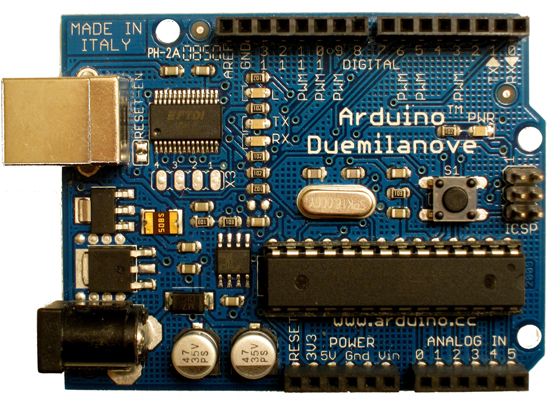
\includegraphics[width=0.3\textwidth,height=3cm,keepaspectratio]{obrazky/emded_arduino_duemilanove}\label{emded_arduino_duemilanove}}
			\hspace*{5mm}
			\subfigure[Arduino Uno]{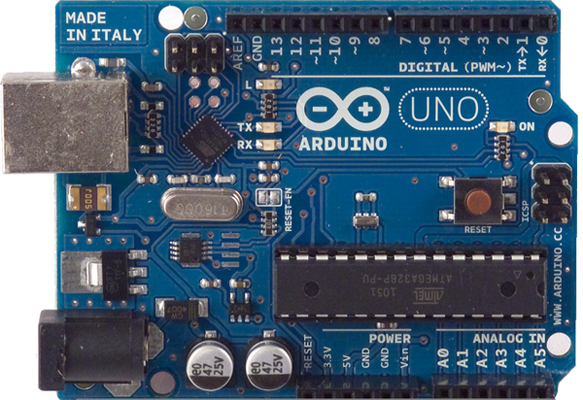
\includegraphics[width=0.3\textwidth,height=3cm,keepaspectratio]{obrazky/emded_arduino_uno}\label{emded_arduino_uno}}
			\hspace*{5mm}
			\subfigure[Arduino Leonardo]{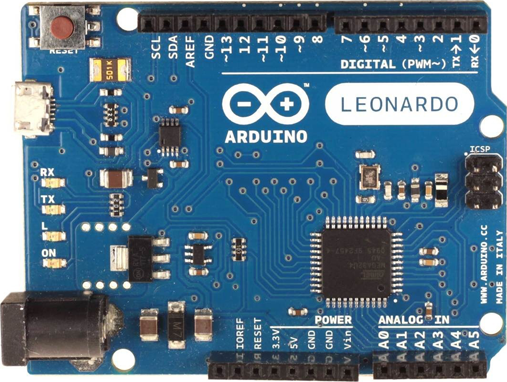
\includegraphics[width=0.3\textwidth,height=3cm,keepaspectratio]{obrazky/emded_arduino_leonardo}\label{emded_arduino_leonardo}}
    \caption{Arduino Duemilanove, Uno a Leonardo}
		\vspace{-10pt}	
\end{figure*}


\newpage
	
					\subsection{Arduino Mega} 
					Arduino Mega je deska pro náročnější projekty. Oproti klasickému Arduinu má~Arduino Mega rychlejší procesor (16\,MHz) a také více vstupních a výstupních pinů. K~dispozici je 54 digitálních pinů, 14 PWM výstupů, 16 analogových vstupů a~4~hardwarové sériové porty. Dále má 256\,KB flash paměti, 8\,KB RAM paměti a 4\,KB EEPROM paměti~\cite{ArduinoMega}.	
			
		\subsection{Arduino Due} 
		Arduino Due je nástupcem Arduino Mega a je to první karta Arduino, na~níž~je~umístěn 32-bitový řadič (32-bitový ARM procesor
		Atmel SAM3X8E). Vysoká taktovací rychlost 84\,MHz ve spojení s celkem 54 I/O piny umožňuje realizaci značně rozsáhlých projektů. K 54 pinům mimo jiné patří 12 PWM výstupů a 12 analogových vstupů, 4 UARTy, 2 I2C a dvojitý digitálně-analogový měnič. Vlastní USB Host poskytuje kartě vedle standardů jako JTAG (Joint Test Action Group), SPI (Serial Peripheral Interface) a Micro USB širší možnosti konektivity~\cite{ArduinoDue}.	

\begin{figure*}[!ht]
    \centering
			\subfigure[Arduino Mega]{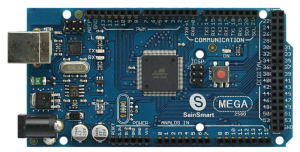
\includegraphics[width=0.45\textwidth,height=3.5cm,keepaspectratio]{obrazky/emded_arduino_mega}\label{emded_arduino_mega}}
			\hspace*{5mm}
			\subfigure[Arduino Due]{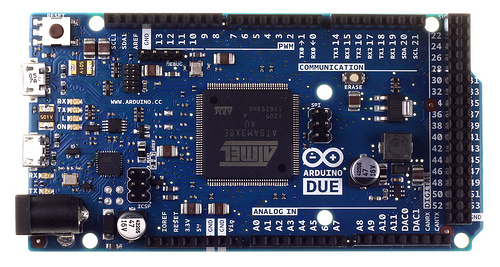
\includegraphics[width=0.45\textwidth,height=3.5cm,keepaspectratio]{obrazky/emded_arduino_due}\label{emded_arduino_due}}
		\caption{Arduino Mega a Due}
		\vspace{-20pt}	
\end{figure*}


	\subsection{Arduino Mini} 
	Arduino Mini je nejmenší oficiální verze Arduina, navržená pro úsporu místa. Daní za malé rozměry je~však absence USB portu. K programování je tedy nutné použít externí USB2Serial převodník. Jeho výkon však nijak nezaostává za většími deskami. Běží na procesoru ATmega328 s taktem 16\,MHz. Pro své malé rozměry je~vhodný k použití například v chytrých vypínačích, či dálkových ovladačích~\cite{ArduinoMini}.	
	
	\subsection{Arduino Micro} 
	Arduino Micro je jedna z desek, která má čip obsahující předprogramovaný převodník ATmega32u4~\cite{ArduinoMicro}.	 
		
	\subsection{Arduino Nano} 
	Arduino Nano navíc obsahuje ještě USB port a převodník~\cite{ArduinoNano}.	
		
\begin{figure*}[!ht]
	\vspace{-10pt}	
    \centering
			\subfigure[Arduino Mini]{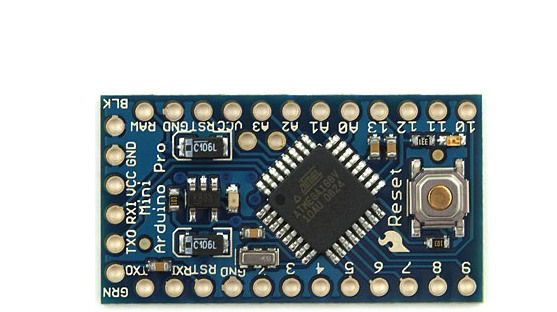
\includegraphics[width=0.3\textwidth,height=3.5cm,keepaspectratio]{obrazky/emded_arduino_mini}\label{emded_arduino_mini}}
			\hspace*{5mm}
			\subfigure[Arduino Micro]{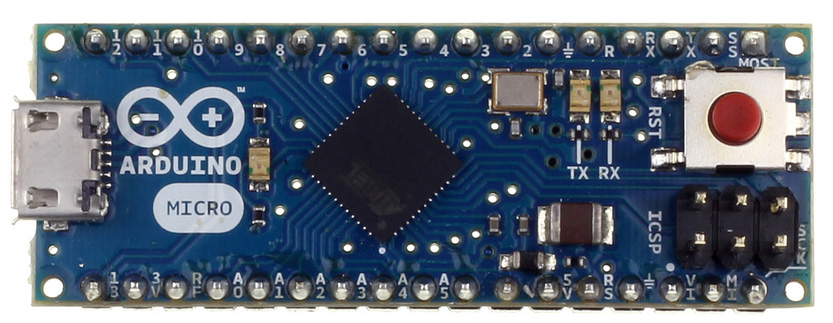
\includegraphics[width=0.3\textwidth,height=3.5cm,keepaspectratio]{obrazky/emded_arduino_micro}\label{emded_arduino_micro}}
			\hspace*{5mm}
			\subfigure[Arduino Nano]{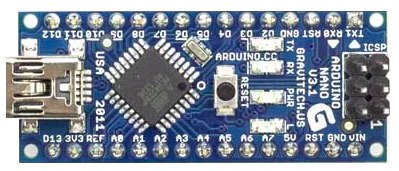
\includegraphics[width=0.3\textwidth,height=3.5cm,keepaspectratio]{obrazky/emded_arduino_nano}\label{emded_arduino_nano}}
		\caption{Arduino Mini, Micro a Nano}
		\vspace{-30pt}	
\end{figure*}
	
		
		\subsection{Arduino Fio} 
		Arduino Fio je přizpůsobená k připojení různých bezdrátových modulů (například ZigBee nebo XBee moduly). Základem je procesor ATmega328P s frekvencí 8\,MHz. Napětí je zde kvůli kompatibilitě s moduly sníženo oproti většině ostatních desek z 5\,V na 3,3\,V~\cite{ArduinoFio}.	
		
	\subsection{Arduino MKR1000}
	Arduino MKR1000 je postavené na čipu ATSAMW25 od Atmelu, který v sobě spojuje ARMové jádro SAMD21 Cortex-M, Wi-Fi čip a šifrovací a autentizační čip ECC508. Tento čip nabízí ECDH (Diffie-Hellman s využitím eliptických křivek) a~ECDSA (Elliptic Curve Digital Signature Algorithm). Dále pak generátor náhodných čísel, unikátní 72bitové sériové číslo nebo SHA-256 s volitelným HMAC.
	
	
	\begin{figure*}[!ht]
    \centering
			\subfigure[Arduino Fio]{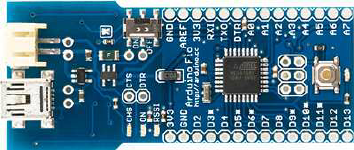
\includegraphics[width=0.33\textwidth,height=3.5cm,keepaspectratio]{obrazky/emded_arduino_fio}\label{emded_arduino_fio}}
			\hspace*{5mm}
			\subfigure[Arduino MKR1000]{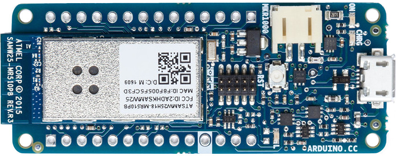
\includegraphics[width=0.33\textwidth,height=3.5cm,keepaspectratio]{obrazky/emded_arduino_mkr1000}\label{emded_arduino_mkr1000}}
		\caption{Arduino Fio a MKR1000}
		\vspace{-30pt}	
\end{figure*}
	
		\subsection{Lilypad Arduino} 
		Lilypad Arduino je postaveno na ATmega168V (energeticky úsporná verze ATmega168) nebo ATmega328V. Je určeno pro wearables projekty, zejména pro implementaci do textilií, kdy jsou spoje vytvořeny pomocí vodivých nití. Není však pratelná. Existuje více variant této desky~\cite{ArduinoLilipad}.	
	
	\subsection{Arduino Yun} 
	Arduino Yun je deska založená na ATmega32u4 (architektura ARM) a Atheros AR9331 (architektiura x86), a umožňuje běh odlehčeného linuxu Linino. Obsahuje softwarový můstek zajišťující komunikaci obou čipů. Procesor Atheros podporuje linuxové distribuce založené na OpenWrt s názvem OpenWrt-Yun. Deska má vestavěný Ethernet a WiFi modul, USB-A port, slot pro MicroSD kartu. Dále disponuje 20 digitálními I/O piny, z toho 7 mohou být použito jako výstupy PWM a 12 jako analogové vstupy~\cite{ArduinoYun}.	

	\begin{figure*}[!ht]
    \centering
			\subfigure[Lilypad Arduino ]{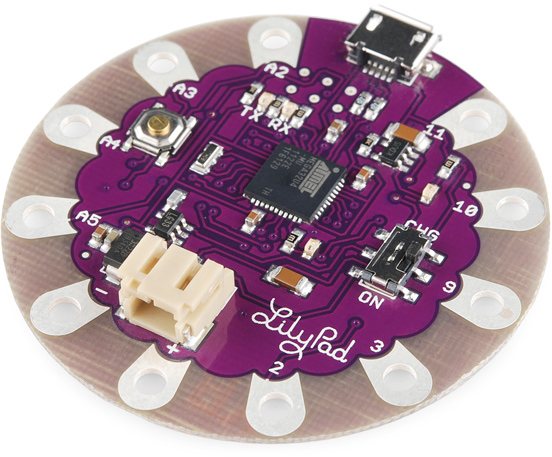
\includegraphics[width=0.55\textwidth,height=3.5cm,keepaspectratio]{obrazky/emded_arduino_lilipad}\label{emded_arduino_lilipad}}
			\hspace*{5mm}
			\subfigure[Arduino Yun ]{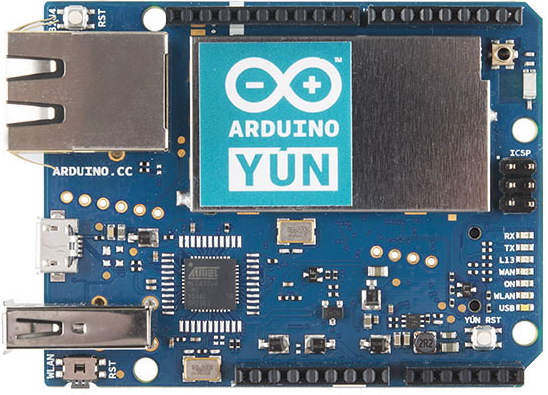
\includegraphics[width=0.35\textwidth,height=3.5cm,keepaspectratio]{obrazky/emded_arduino_yun}\label{emded_arduino_yun}}
			\caption{Lilypad Arduino a Arduino Yun}
			\vspace{-10pt}	
\end{figure*}
	
%%%%%%%%%%%%%%%%%%%%%%%%%%%%%%%%%%%%%%%%%%%%%%%%%%%%%%%%%%%%%%%%%%%%%%%%%%%%%%%%%%%%%%%%%%%%%%%%%%%%%%%%%%%%%%%%%
%%%%%%%%%%%%%%%%%%%%%%%%%%%%%%%%%%%%%%%%%%%%%%%%%%%%%%%%%%%%%%%%%%%%%%%%%%%%%%%%%%%%%%%%%%%%%%%%%%%%%%%%%%%%%%%%%
%%%%%%%%%%%%%%%%%%%%%%%%%%%%%%%%%%%%%%%%%%%%%%%%%%%%%%%%%%%%%%%%%%%%%%%%%%%%%%%%%%%%%%%%%%%%%%%%%%%%%%%%%%%%%%%%%
%%%%%%%%%%%%%%%%%%%%%%%%%%%%%%%%%%%%%%%%%%%%%%%%%%%%%%%%%%%%%%%%%%%%%%%%%%%%%%%%%%%%%%%%%%%%%%%%%%%%%%%%%%%%%%%%%
%%%%%%%%%%%%%%%%%%%%%%%%%%%%%%%%%%%%%%%%%%%%%%%%%%%%%%%%%%%%%%%%%%%%%%%%%%%%%%%%%%%%%%%%%%%%%%%%%%%%%%%%%%%%%%%%%
%%%%%%%%%%%%%%%%%%%%%%%%%%%%%%%%%%%%%%%%%%%%%%%%%%%%%%%%%%%%%%%%%%%%%%%%%%%%%%%%%%%%%%%%%%%%%%%%%%%%%%%%%%%%%%%%%

\section{Arduino klony}
\label{KapArduinoKlony}

	Jelikož je projekt Arduino open-source, vzniklo množství klonů od dalších firem i jednotlivců. Klony jsou s původním Arduinem kompatibilní, ve většině případů konfigurací odpovídají některému z Arduino modelu, většinou Arduino UNO. Kity, které nemají shodné rozložení pinů neumožňují připojení Arduino shieldů. V této podkapitole je uveden krátký přehled těch nejznámějších. Rozsáhlý přehled kompatibilních klonů lze nalézt na oficiálních stránkách Arduina~\cite{ArduinoClonesWeb}.
	
	\subsection{Freeduino} 
	Freeduino je klon Arduina, vycházející z Arduino Duemilanove.
	
	\subsection{LABduino} 
	LABduino je český klon Arduina vytvořený z otevřené elektronické stavebnice MLAB.
	
	\subsection{Arduelo Libero}	
	Arduelo Libero je mírně vylepšený český free klon Arduino Duemilanove.
	
	\subsection{Bare Bones Board} 
	Bare Bones Board je kompatibilní deska, tvarově nepřipomínající žádný Arduino produkt. Kvůli rozložení pinů nepodporuje shieldy. Vyráběná a prodávaná jako kit firmou Modern Device Company.
	
	\subsection{Freaduino} 
	Freaduino je kompatibilní deska, tvarově shodná s Arduino UNO, vyráběná a prodávaná firmou ElecFreak jako kit The Freaduino Uno. Podporuje 3,3\,V logiku a~napájení. Má piny na připojení modulů (XBee). Napájecí piny zvládají zátěž až 2\,A.

	\begin{figure*}[!ht]
	\vspace{-10pt}	
    \centering
			\subfigure[Bare Bones Board]{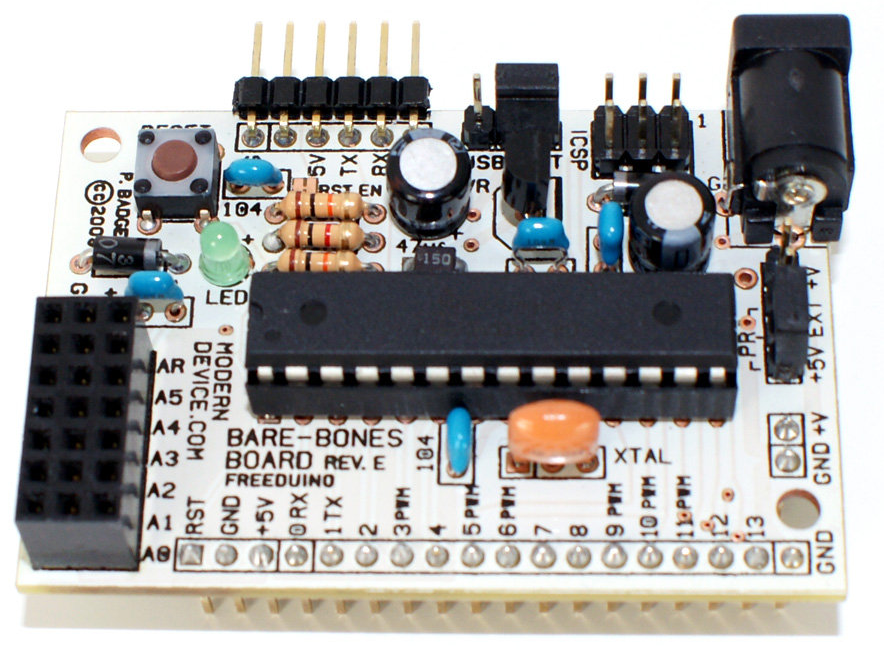
\includegraphics[width=0.45\textwidth,height=3.5cm,keepaspectratio]{obrazky/embed_barebones}\label{emded_barebones}}
			\hspace*{5mm}
			\subfigure[Freaduino]{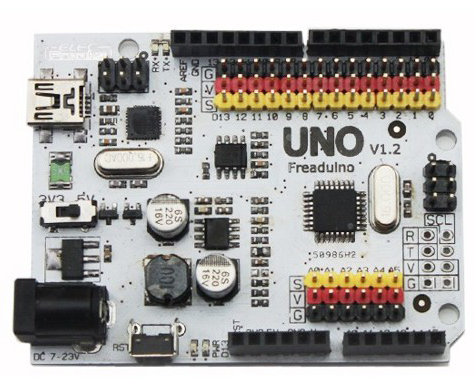
\includegraphics[width=0.45\textwidth,height=3.5cm,keepaspectratio]{obrazky/embed_freaduino}\label{emded_freaduino}}
					\caption{Bare Bones Board a Freaduino}
					\vspace{-20pt}	
	\end{figure*}	
	
	\subsection{Runtime} 
	Runtime je kompatibilní deska, tvarově nepřipomínající žádný Arduino produkt. Kvůli rozložení pinů nepodporující shieldy. Vyráběná a prodávaná jako kit firmou NKC Electronics.
	
	\subsection{Nanode} 
	Nanode je kompatibilní deska, tvarově nepřipomínající žádný Arduino produkt. Tvarově připomíná Arduino UNO, rozložení pinů je kompatibilní.
	
	\subsection{Seeeduino} 
	Seeeduino je kompatibilní deska, vzhledem připomínající Arduino UNO, parametricky shodná s Arduino Mega.
	
	\subsection{Teensy}
	Teensy je kompletní vývojový mikrokontrolérový systém na velmi malé desce bez~osazených pinů, který je schopen realizovat mnoho typů projektů. Softwarově je~kompatibilní s Arduinem, programuje se však pomocí doplňku do Arduino IDE nebo pomocí WinAVR~\cite{ArduinoTeensy}.
	
	\subsection{Diavolino} 
	Diavolino je free klon Arduina, vzhledově i parametricky podobný Arduino UNO, bez~vyvedených konektorů. Vyráběná a prodávané jako kit firmou Evil Mad Scientist.
		
	\subsection{Boarduino} 
	Boarduino je levnější klon Arduina Diecimila s piny pro zapojení rovnou do nepájivého pole.

\begin{figure*}[!ht]
    \centering
			\subfigure[Diavolino]{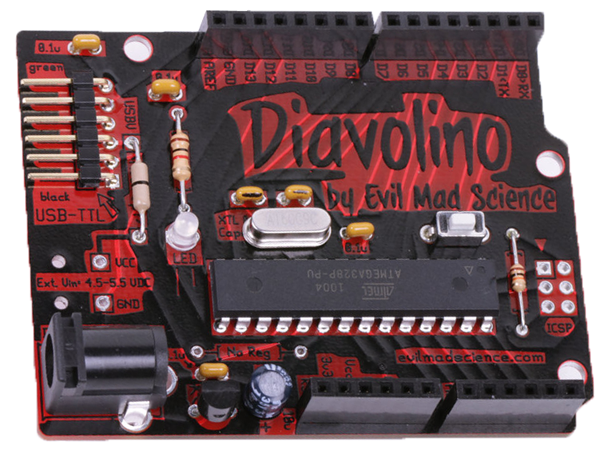
\includegraphics[width=0.45\textwidth,height=3.5cm,keepaspectratio]{obrazky/embed_diavolino}\label{emded_diavolino}}
			\hspace*{5mm}
			\subfigure[Boarduino]{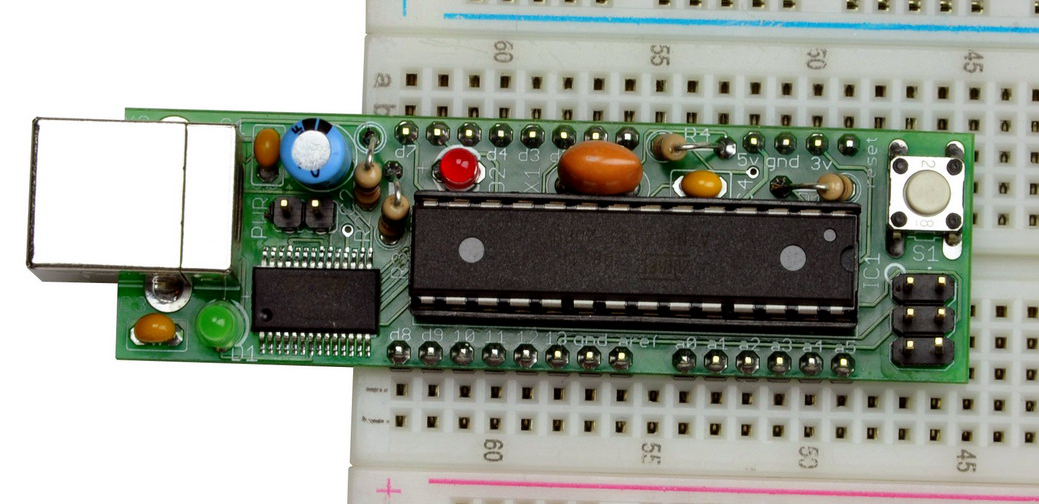
\includegraphics[width=0.45\textwidth,height=3.5cm,keepaspectratio]{obrazky/embed_boarduino}\label{emded_boarduino}}
					\caption{Diavolino a Boarduino}
					\vspace{-30pt}	
	\end{figure*}	

%%%%%%%%%%%%%%%%%%%%%%%%%%%%%%%%%%%%%%%%%%%%%%%%%%%%%%%%%%%%%%%%%%%%%%%%%%%%%%%%%%%%%%%%%%%%%%%%%%%%%%%%%%%%%%%%%
%%%%%%%%%%%%%%%%%%%%%%%%%%%%%%%%%%%%%%%%%%%%%%%%%%%%%%%%%%%%%%%%%%%%%%%%%%%%%%%%%%%%%%%%%%%%%%%%%%%%%%%%%%%%%%%%%
%%%%%%%%%%%%%%%%%%%%%%%%%%%%%%%%%%%%%%%%%%%%%%%%%%%%%%%%%%%%%%%%%%%%%%%%%%%%%%%%%%%%%%%%%%%%%%%%%%%%%%%%%%%%%%%%%
%%%%%%%%%%%%%%%%%%%%%%%%%%%%%%%%%%%%%%%%%%%%%%%%%%%%%%%%%%%%%%%%%%%%%%%%%%%%%%%%%%%%%%%%%%%%%%%%%%%%%%%%%%%%%%%%%
%%%%%%%%%%%%%%%%%%%%%%%%%%%%%%%%%%%%%%%%%%%%%%%%%%%%%%%%%%%%%%%%%%%%%%%%%%%%%%%%%%%%%%%%%%%%%%%%%%%%%%%%%%%%%%%%%
%%%%%%%%%%%%%%%%%%%%%%%%%%%%%%%%%%%%%%%%%%%%%%%%%%%%%%%%%%%%%%%%%%%%%%%%%%%%%%%%%%%%%%%%%%%%%%%%%%%%%%%%%%%%%%%%%

\section{RaspberryPi}
\label{KapRaspi}

RaspberryPi reprezentuje jednodeskový počítač o velikosti zhruba platební karty. Byl vyvinut v roce 2012 s cílem podpořit výuku informatiky a seznámit studenty s~řízením různých zařízení přes počítač~\cite{Raspi}. 

Primárním operačním systémem je Linux, k dispozici je několik jeho distribucí, případně lze použít Windows 10 IoT Core. Na rozdíl do Arduina obsahuje RaspberryPi plnohodnotný operační systém, ARM mikrokontrolér, USB pro připojení myši a klávesnice, Ethernet konektor pro připojení sítě, grafický výstup HDMI (High-Definition Multimedia Interface) a kompozitní video, DSI (Display Serial Interface) pro připojení displeje, CSI (Camera Serial Interface) pro připojení kamery a čtečku pamětových karet, tedy působí spíše jako menší počítač, než vývojová platforma. 

Všechny další rozšiřující sběrnice (UART, I2C, SPI, PWM, digitální vstup a~výstup, analogový vstup) jsou vyvedeny do 26 nebo 40 pinového GPIO konektoru. Na~rozdíl od Arduina je možné RaspberryPi pomocí GPIO kontaktů použít nejen k ovládání různých zařízení, ale i~k~samotnému vývoji příslušných aplikací. Lze ho také použít jako multimediální přehrávač videa nebo hudby nebo i jen pro přístup k Internetu.

RaspberryPi stejně jako Arduino podporuje připojení rozšiřujících karet:

\begin{itemize}
	\item \textbf{Pi T-Cobbler} je pasivní elektronický přípravek, který se k RaspberryPi připojuje pomocí 40 žilového plochého kabelu a slouží k vyvedení pinů do vývojové desky breadboard. Zde na konektorové desce jsou již jednotlivé piny popsány.
\item \textbf{Gertboard} je rozšiřující deska autora Gerta Van Loo, který rozšiřuje I/O možnosti RaspberryPi. K ní se připojuje pomocí 40 žilového plochého kabelu a~rozšiřuje možnosti o 8/10/12-bitový dvoukanálový D/A převodník, 10-bitový dvoukanálový A/D převodník, obvody pro řízení motoru, předprogramovaný Atmel AVR ATmega 328P, 6 výstupů s otevřeným kolektorem a dalších 12 IO pinů~\cite{GertBoard}.  
\item \textbf{UniPi} je rozšiřující deska která rozšiřuje I/O možnosti RaspberryPi. K~ní~se~připojuje pomocí 26 žilového plochého kabelu a dle typu připojeného UniPi zařízení poskytuje I/O funkce navíc. Rozšiřujícími moduly UniPi se bude blíže zabývat následující kapitola (Kap.~\ref{KapUnipi}).
\item \textbf{RaspberryPi to Arduino Shield} je rozšiřující deska, která umožňuje propojení RasbperryPi a vybraných modelů Arduino.
\end{itemize}
Samozřejmě lze k Arduinu připojit i samotné moduly nebo senzory, přímým připojením na dané piny GPIO konektoru. Je však třeba dbát na to, že RaspberryPi pracuje s 3,3\,V logikou, zatímco například Arduino pracuje s 5\,V logikou. Popis GPIO konektoru včetně možností připojení je součástí Kap.~\ref{KapGPIO}.

	\subsection{RaspberryPi}
	Původní model RaspberryPi byl zveřejněn v únoru roku 2012. Obsahuje jednojádrový procesor o frekvenci 700\,MHz. U této verze existovaly tři modely~\cite{RaspiOne}:
	
		\begin{itemize}
		\item \textbf{Model A+} je odlehčená levná verze modelu B. Nemá žádný pamětový slot. Disponuje 256\,MB RAM. Neobsahuje USB port. Má 40 GPIO pinů.
		\item \textbf{Model B} byl původní RaspberryPi. Má slot na SD kartu. Disponuje 512\,MB RAM. Obsahuje 1 USB port. Má 26 GPIO pinů. Má samostatný výstup kompozitního videa.
		\item \textbf{Model B+} obsahuje slot na MicroSD kartu. Disponuje 512\,MB RAM. Obsahuje 2 USB porty. Má 40 GPIO pinů.
	\end{itemize}
	
\begin{figure*}[!ht]
    \centering
			\subfigure[Model A+]{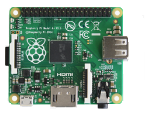
\includegraphics[height=3.5cm,keepaspectratio]{obrazky/embed_raspi_1a}\label{embed_raspi_1a}}
			\hspace*{2mm}
			\subfigure[Model B]{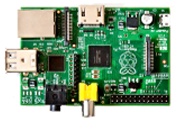
\includegraphics[height=3.5cm,keepaspectratio]{obrazky/embed_raspi_1b}\label{embed_raspi_1b}}
			\hspace*{2mm}
			\subfigure[Model B+]{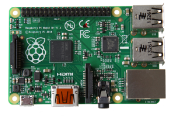
\includegraphics[height=3.5cm,keepaspectratio]{obrazky/embed_raspi_1bp}\label{embed_raspi_1bp}}
		\caption{RaspberryPi prvních verzí}
\end{figure*}
	
	\subsection{RaspberryPi 2}
	RaspberryPi 2 je pokračováním RaspberryPi, které přináší zejména vyšší výkon. Díky čtyřjádrovému procesoru BCM2836 o taktu 900\,MHz by měl být 3-6× rychlejší než jeho předchůdce. Tento model disponuje 1\,GB paměti a má 4 USB porty~\cite{RaspiTwo}.


\subsection{RaspberryPi 3}
		RaspberryPi 3, dostupný od roku 2016 je vybaven čtyřjádrovým 64bitovým procesorem ARM Cortex-A53 o taktu 1,2\,GHz. Oproti předchozímu modelu přináší integraci WiFi a Bluetooth modulů přímo na desce a měl by být dvakrát rychlejší~\cite{RaspiThree}.
		
\subsection{RaspberryPi Zero}
		RaspberryPi Zero je nejúspornější varianta RaspberryPi, ideální pro použití v IoT. Vychází z modelu A+, ve srovnání s ním nabízí procesor s frekvencí 1\,GHz a 512\,MB paměti. Má přibližně poloviční velikost, nemá však vyvedené piny GPIO konektoru, USB konektory má ve verzi micro a HDMI ve verzi mini~\cite{RaspiZero}.

\begin{figure*}[!ht]
    \centering
			\subfigure[RaspberryPi 2]{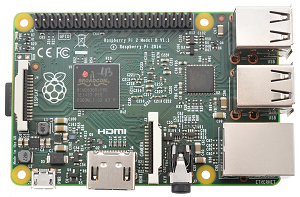
\includegraphics[width=0.3\textwidth,height=3.5cm,keepaspectratio]{obrazky/embed_raspi_2}\label{embed_raspi_2}}
			\hspace*{5mm}
			\subfigure[RaspberryPi 3]{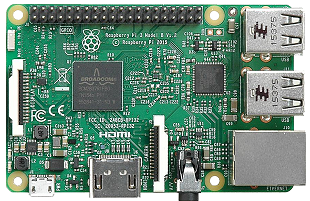
\includegraphics[width=0.3\textwidth,height=3.5cm,keepaspectratio]{obrazky/embed_raspi_3}\label{embed_raspi_3}}
			\hspace*{5mm}
			\subfigure[RaspberryPi Zero]{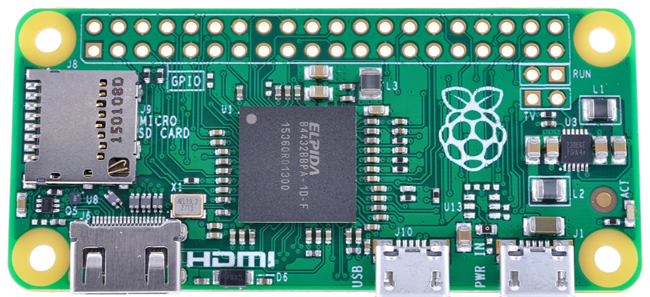
\includegraphics[width=0.3\textwidth,height=3.5cm,keepaspectratio]{obrazky/embed_raspi_zero}\label{embed_raspi_zero}}
		\caption{RaspberryPi následujících verzí}
\end{figure*}


%%%%%%%%%%%%%%%%%%%%%%%%%%%%%%%%%%%%%%%%%%%%%%%%%%%%%%%%%%%%%%%%%%%%%%%%%%%%%%%%%%%%%%%%%%%%%%%%%%%%%%%%%%%%%%%%%
%%%%%%%%%%%%%%%%%%%%%%%%%%%%%%%%%%%%%%%%%%%%%%%%%%%%%%%%%%%%%%%%%%%%%%%%%%%%%%%%%%%%%%%%%%%%%%%%%%%%%%%%%%%%%%%%%
%%%%%%%%%%%%%%%%%%%%%%%%%%%%%%%%%%%%%%%%%%%%%%%%%%%%%%%%%%%%%%%%%%%%%%%%%%%%%%%%%%%%%%%%%%%%%%%%%%%%%%%%%%%%%%%%%
%%%%%%%%%%%%%%%%%%%%%%%%%%%%%%%%%%%%%%%%%%%%%%%%%%%%%%%%%%%%%%%%%%%%%%%%%%%%%%%%%%%%%%%%%%%%%%%%%%%%%%%%%%%%%%%%%
%%%%%%%%%%%%%%%%%%%%%%%%%%%%%%%%%%%%%%%%%%%%%%%%%%%%%%%%%%%%%%%%%%%%%%%%%%%%%%%%%%%%%%%%%%%%%%%%%%%%%%%%%%%%%%%%%
%%%%%%%%%%%%%%%%%%%%%%%%%%%%%%%%%%%%%%%%%%%%%%%%%%%%%%%%%%%%%%%%%%%%%%%%%%%%%%%%%%%%%%%%%%%%%%%%%%%%%%%%%%%%%%%%%

\section{RaspberryPi klony}
\label{KapRaspiKlony}

Vzrůstající popularita RaspberryPi dala stejně jak u Arduina vzniknout celé řadě klonů. Tyto klony odvozují ze základního sestavení RaspberryPi a určitým způsobem ho rozřišují. Jelikož označení „RaspberryPi“ je registrovanou ochrannou známkou, mají podobně navžené počítače odvozené názvy, jako BananaPi a~OrangePi. Zmíněné klony patří k nejznámějším a každý z nich již existuje v několika verzích, v této podkapitole budou představeny ty nejznámější s uvedením jejich hlavních odchylek od RaspberryPi.

%%% ======================================= BANANA PI ============================== %%%
	\subsection{BananaPi}
		Původní BananaPi, ze kterého vychází řada dalších modelů, je malý jednodeskový počítač, který se na první pohled podobá RaspberryPi.  Obsahuje dvoujádrový procesor a 512\,MB RAM. Na rozdíl od RaspberryPi obsahuje BananaPi také SATA řadič, mikrofon, který je připájen přímo na desce, gigabitový Ethernet, USB 2.0 OTG (On The Go), IR (Infrared Radiation) přijímač, tlačítko reset a power. Počítač podporuje SATA disky až~do~velikosti 2\,TB. GPIO konektor je vždy kompatibilní s některou verzi RaspberryPi. Za~výrobou všech počítačů BananaPi stojí čínská firma SinoVoip CO., Limited~\cite{BananaPi}.
		
	\textbf{BananaPi BPI-M2} je klon RaspberryPi 2, obsahuje taktéž čtyřjádrový procesor běžící na 1 GHz, má již integrovanou WiFi (Wireless Fidelity), ale neobsahuje SATA (Serial Advanced Technology Attachment) port.
	
	\textbf{BananaPi BPI-M3} obsahuje osmijádrový procesor 1,8\,GHz s 2\,GB RAM, dále zahrnuje WiFi b/g/n a integrované Bluetooth 4. Obsahuje SATA port.
	
	\textbf{BananaPi BPI-M64} obsahuje oproti modelu M3 čtyřjádrový 64 bitový SoC procesor Allwinner A64.
	
	%%% ======================================= ORANGE PI ============================== %%%
	\subsection{OrangePi}
	OrangePi je alternativa pro RaspberryPi vznikající v posledních dvou letech. Všechny modely jsou založeny na architektuře ARM Cortex-A7 s SoC Allwinner H3 s čtyřjádrovým CPU, výjimkou jsou OrangePi a OrangePi Mini, které mají SoC Allwinner A20 s dvojádrovým CPU. Grafickým čipem je u všech modelů ARM Mali-400 MP2. Všechny modely podporují HDMI CEC~\cite{OrangePi}.

		\textbf{OrangePi} je základní model z rodiny OrangePi, obsahuje čtyřjádrový procesor Allwinner A20 na 1\,GHz a 1\,GB RAM. Oproti RaspberryPi má navíc pouze mikrofon, IR port, USB OTG, ale nemá DSI rozhraní.
		
		\textbf{OrangePi Plus } má procesory běžící na 1,6\,GHz, 1\,GB RAM a 8\,GB EMMC Flash. Oproti RaspberryPi má gigabitový Ethernet, integrovaný mikrofon, USB-OTG konektor, integrovaný WiFi modul, IR přijímač. Obsahuje SATA port, který je připojený přes USB převodník.
		
		\textbf{OrangePi Plus2} oproti předchozí verzi došlo k navýšení pamětí na 2\,GB RAM a 16\,GB eMMC (embedded MultiMedia Card) Flash a doplnění CSI (Camera Serial Interface) konektoru.
		
		\textbf{OrangePi One} vznikla jako reakce na odlehčenou verzi RaspberryPi Zero. Jedná se o čtyřjádrový procesor na frekvenci 1,2\,GHz postavený na čipu ARM Cortex-A7 s grafickým čipem Mali400 MP2. Operační paměť je 512\,MB. K dispozici je pouze 10/100\,Mbps Ethernet a jeden port USB 2.0.

	\begin{figure*}[!ht]
	\vspace{-10pt}
    \centering
			\subfigure[BananaPi BPI-M2]{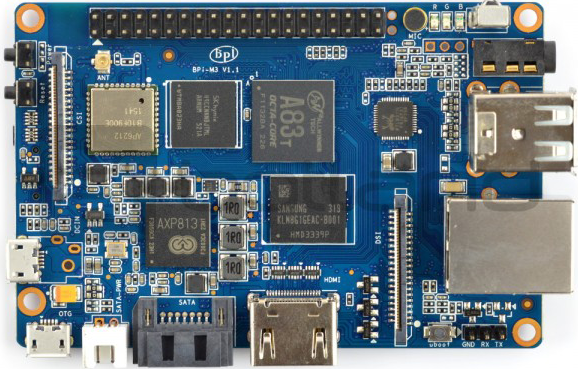
\includegraphics[height=4cm]{obrazky/embed_bananapim2}\label{embed_bananapim2}}
			\hspace*{5mm}
			\subfigure[OrangePi Plus2]{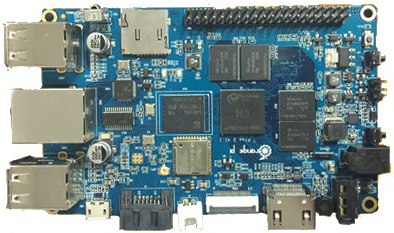
\includegraphics[height=4cm]{obrazky/embed_orangepiplus2}\label{embed_orangepiplus2}}
			\caption{BananaPi BPI-M2 a OrangePi Plus2}
			\vspace{-10pt}	
\end{figure*}
	
	

%%% ======================================= CUBIE BOARD ============================== %%%
	\subsection{CubieBoard}
	\label{KapCubie}
			CubieBoard je alternativou k RaspberryPi z roku 2012. Ačkoliv jsou vzhledově i~parametricky velmi podobné, není Cubieboard s RaspberryPi kompatibilní. Jsou postaveny na AllWinner A10 SoC čipu. Výrobce poskytuje vlastní sadu modulů a rozšiřujících desek. Cubieboardy poskytují pinové rozhraní, obsahující základní sběrnice (I2C, SPI, UART) ale i rozšiřující jako LVDS (Low-Voltage Differential Signaling). Desky obsahují navíc SATA konektor~\cite{CubieBoards}.
	
	\textbf{CubieBoard 1} je výkonná nízkopříkonová deska s ARM A8 o taktu 1\,GHz s~1\,GB RAM, 4\,GB NAND flash a Mali400 GPU. Obsahuje LAN port a dvojici USB portů. Deska má 96 pinů, které zahrnují sběrnice GPIO, I2C, UART, LVDS (Low Resolution Analog to Digital Converter), PWM, SPI, CSI, VGA a jiné. Dále obsahuje 100Mbps Ethernet a dva USB HOST porty, mini USB OTG, čtečku micro SD, HDMI, IR, line in, line out a SATA port.
	
	\textbf{CubieBoard 2} představuje nástupce CubieBoardu1, je s ním zpětně kompatibilní a~od~předchozí verze se liší pouze dvoujádrovým provedením CPU a GPU.
		
	\textbf{CubieBoard 3} oproti předchozím verzím přínaší vylepšení jako 2\,GB RAM, 8\,GB NAND flash, VGA konektor přímo na desce, gigabitový Ethernet, WiFi a~Bluetooth integrované přímo na desce. Pinové rozhranní je zde redukováno na 54 pinů obsahující I2S (Inter-Integrated Sound), I2C, SPI, CVBS (Color Video Blanc Sync), UART, PWM a GPIO.
	
		\textbf{CubieBoard 4} je nástupce CubieBoardu 3, je zpětně kompatibilní a oproti předchůdci přináší čtyřjádrové CPU ARM A15x a GPU PowerVR G6230. Dále má microUSB 3.0 OTG a audio konektory umístěné přímo na desce.
		
			\textbf{CubieBoard 5 }nabízí osmijádrový procesor Allwinner H8, který doplňují 2\,GB RAM. Navíc oproti předchozím verzím má kromě HDMI i DP (Display Port), přináší taktéž konektor pro připojení externí baterie. Došlo k navýšení GPIO pinů na 70, které navíc přináší LRADC (Low Resolution Analog to Digital Converter) a PS2 (Personal System/2). SATA konektor pomocí speciální desky podporuje připojení dvou SATA disků s podporou RAIDu.
		
CubieBoardy již poskytují dostatečný výkon pro embeeded zařízení, přináší oproti RaspberryPi mnoho rozšiřujících sběrnic, avšak pro nedostatečnou podporu či zastoupení v evropských zemí a velmi častou nedostupnost webu výrobce, včetně dostupnosti anglické dokumentace pro  programování jednotlivých rozhraní, není moc vhodná pro IoT. Hodí se spíše pro aplikace jako multimediální centrum či nízkonákladový počítač. 	

%%% ======================================= UP BOARD ============================ %%%

\subsection{UpBoard}
		UpBoard představuje miniaturní jednodeskový počítač na platformě Intel s čtyřjádrovým procesorem Intel Atom. Vzhledově je velice podpobný RaspberryPi 3. 
		Tento počítač obsahuje čtyřjádrový procesor Intel Atom x5-Z8300 na frekvenci 1,84 GHz s~TDP 2\,W. Obsahuje 1\,GB RAM a 16\,GB flash eMMC (Embedded MultiMedia Card). 40 pinové rozhraní je totožné jako u RaspberryPi 2 s níž je částečně kompatibilní. Navíc obsahuje gigabitový Ethernet port, 5 USB 2.0 a jedno USB 3.0. Čip má hardwarovou podporu šifrování AES (Advanced Encryption Standard), je tedy vhodný pro IoT projekty s vyšším zabezpečením. Podporuje Android 5.0, Linux či Windows 10 IoT Core. Dokumentace pro programování GPIO v současnosti neexistuje, dokumentaci tvoří pouze popis GPIO konektoru~\cite{UpBoard}.

	\begin{figure*}[!ht]
	\vspace{-10pt}	
    \centering
			\subfigure[CubieBoard1]{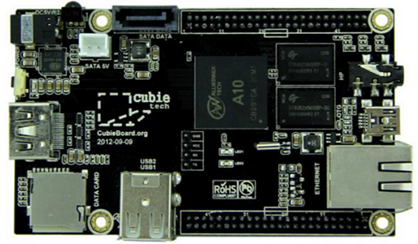
\includegraphics[height=4cm]{obrazky/embed_cubie_1}\label{embed_cubie_1}}
			\hspace*{5mm}
			\subfigure[UpBoard1]{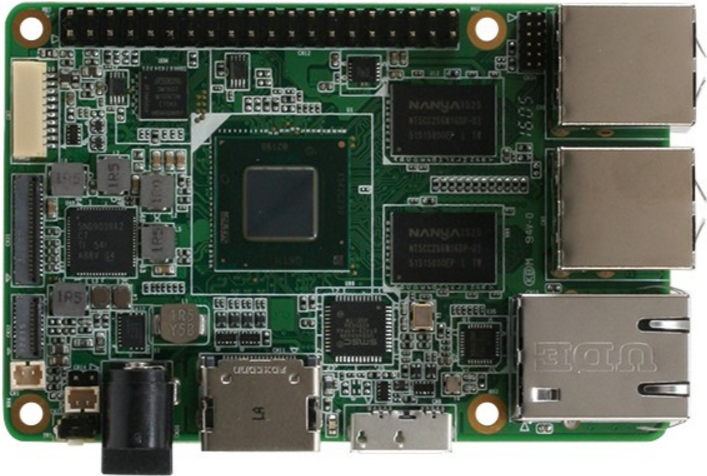
\includegraphics[height=4cm]{obrazky/embed_upboard}\label{embed_upboard}}
			\caption{CubieBoard1 a UpBoard1}
			\vspace{-10pt}	
\end{figure*}
		

%%% ======================================= PINE64 ============================== %%%
	\newpage{}
	\subsection{PINE64}
Pine64 je rodina tří jednodeskových počítačů společnosti PINE64. Tyto počítače byly navrženy tak, aby konkurovaly RaspberryPi ve výkonu a ceně. Všechny verze obsahují 64bitový čtyřjádrový procesor 1,152\,GHz Cortex-A53 a liší se pouze velikostí operační paměti a použitelným operačním systémem. Oproti RaspberryPi obsahují gigabitový Ethernet, WiFi, Bluetooth a port pro připojení dotykového panelu. Mají GPIO konektor shodný s danou verzi Raspberry, jsou s ní tedy do jisté míry kompatibilní. Zvlášností těchto desek je Eulerova sběrnice, která navyšuje počty sběrnic SPI, UART, GPIO~\cite{Pine64}.

\textbf{PINE A64 512MB} má 512\,MB paměti a podporuje pouze Arch Linux a Debian Linux.

\textbf{PINE A64+ 1GB} má 1\,GB paměti a podporuje i Android, Remix OS, Ubuntu a Windows IoT.

\textbf{PINE A64+ 2GB} má oproti předchozí verzi 2\,GB operační paměti.

	\begin{figure*}[!ht]
    \centering
			\subfigure[PINE A64+ 2GB]{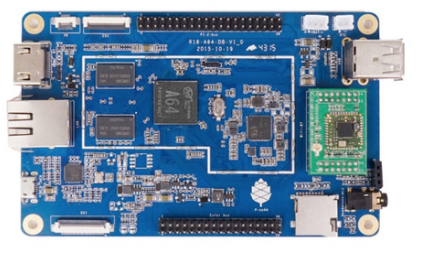
\includegraphics[height=4cm]{obrazky/embed_pine}\label{embed_pine}}
			\hspace*{5mm}
			\subfigure[HardKernel Odroid-C2]{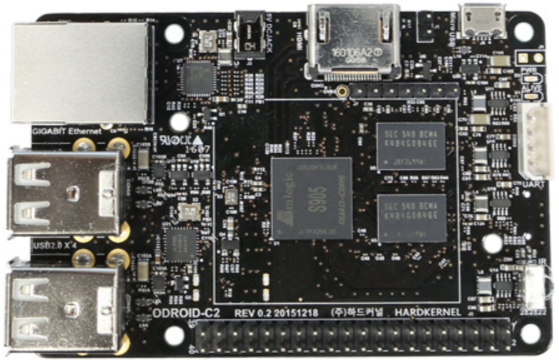
\includegraphics[height=4cm]{obrazky/embed_odroidc2}\label{embed_odroidc2}}
			\caption{PINE A64+ 2GB a HardKernel Odroid-C2}
			\vspace{-10pt}
\end{figure*}

%%% ======================================= ODROID ============================== %%%
\newpage{}
\subsection{HardKernel Odroid}
	\label{KapKernel}
ODROID je řada jednodeskových počítačů od společnosti HardKernel. Název je odvozen z \textbf{O}pen An\textbf{droid}, ale podporovány jsou i linuxové distribuce. Desky disponují 40 pinovým GPIO kompatibilním s RaspberryPi, ale open-source již nejsou. Desky jsou postaveny na SoC platformě Samsung Exynos. Zvláštností desek je sériové rozhraní s 1,8\,V~\cite{HardKernel}.
	
	\textbf{ODROID-C1} je reakcí na RaspberryPi 1. Nabízí čtyřjádrové SoC Cortex A5 s frekvencí 1,5\,GHz a 1\,GB RAM. Dále má gigabitový Ethernet a připojení flash úložiště typu eMMC. 

	\textbf{ODROID-C2} je reakcí na RaspberryPi 3. Obsahuje čtyřjádrový 64bitový procesor ARMv8 taktovaný na 2\,GHz, 2\,GB paměti a gigabitový Ethernet. Má podporu sběrnice I2S. Hlavní změnou je podpora HDMI 2.0 a schopnost přehrávat 4K video ve formátu H.265. Podporuje Ubuntu 16.04 nebo Android 5.1. 
	
	\textbf{ODROID-XU4} je výkonejší řada desek, obsahují čtyřjádrový procesor Samsung Exynos5 ARM Cortex-A15 na frekvenci 2\,GHz a čtyřjádrový procesor Cortex-A7 Quad 1,3\,GHz, bohužel vzhledem k výkonu je zde již aktivní chlazení. Deska disponuje grafickým čipem Mali-T628 MP6 a 2\,GB RAM paměti.

	
%%% ======================================= BeagleBoard ============================== %%%
\subsection{BeagleBoard }
BeagleBoard je skupina jednodeskových počítačů produkovaných společností Texas Instruments, navržených na čipu Texas Instrument's OMAP3530 SoC, ten obsahuje ARM Cortex-A8 CPU, který může provozovat Linuxové distribuce, BSD nebo Android. Desky obsahují dva 46pinové GPIO konektory, oproti ostatním přináší podporu CAN (Controller Area Network) sběrnice. Výrobce poskytuje vlastní řadu kompatibilních rozšiřujicích desek, nazýva je \uv{capes} a současně lze připojit až~4~takovéto desky. Výhodou desek je jejich nízká spotřeba, využívají maxikmálně 2\,W elektrické energie a mohou být napájeny i ze samostatného napájení. Vzhledem k nízké spotřebě energie nejsou nutné žádné přídavné chladiče~\cite{BeagleBone}.

\textbf{BeagleBoard} obsahuje procesor Sitara ARM Cortex-A8 na frekvenci 720\,MHz a disponuje dle revize 128 nebo 256\,MB RAM. Obsahuje 256\,MB NAND paměti.

\textbf{BeagleBone} obsahuje procesor Sitara ARM Cortex-A8 na frekvenci 720\,MHz a~disponuje 256\,MB RAM.

\textbf{BeagleBoard-X15} je založen na šestiádrovém procesoru Sitara AM5728 s dvěma jádry ARM Cortex-A15 na frekvenci 1,5\,GHz a dvěma jádry ARM Cortex-M4 na frekvenci 212\,MHz a dvěma jádry TI C66x DSP na frekvenci 700\,MHz. Disponuje 2\,GB RAM. Použitý procesor přináší podporu HDMI 2.1, gigabitového Ethernetu a grafického dvoujádrového čipu SGX544 na frekvenci 532\,MHz. 

	\begin{figure}[!ht]
  \begin{center}
    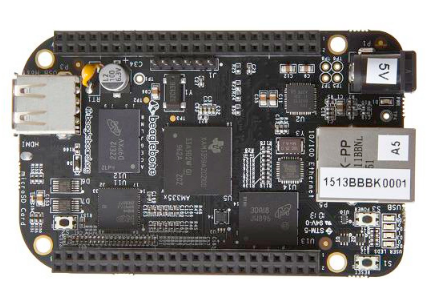
\includegraphics[height=4cm]{obrazky/embed_beaglebone_black}
  \end{center}
	\vspace{-20pt}
  \caption{BeagleBone Black~\cite{BeagleBone}}
\end{figure}

\textbf{BeagleBone Black} má oproti předchůdci zvýšenou pamět na 512\,MB, frekvenci procesoru na 1\,GHz a 2\,GB eMMC flash paměti.

%%%%%%%%%%%%%%%%%%%%%%%%%%%%%%%%%%%%%%%%%%%%%%%%%%%%%%%%%%%%%%%%%%%%%%%%%%%%%%%%%%%%%%%%%%%%%%%%%%%%%%%%%%%%%%%%%
%%%%%%%%%%%%%%%%%%%%%%%%%%%%%%%%%%%%%%%%%%%%%%%%%%%%%%%%%%%%%%%%%%%%%%%%%%%%%%%%%%%%%%%%%%%%%%%%%%%%%%%%%%%%%%%%%
%%%%%%%%%%%%%%%%%%%%%%%%%%%%%%%%%%%%%%%%%%%%%%%%%%%%%%%%%%%%%%%%%%%%%%%%%%%%%%%%%%%%%%%%%%%%%%%%%%%%%%%%%%%%%%%%%
%%%%%%%%%%%%%%%%%%%%%%%%%%%%%%%%%%%%%%%%%%%%%%%%%%%%%%%%%%%%%%%%%%%%%%%%%%%%%%%%%%%%%%%%%%%%%%%%%%%%%%%%%%%%%%%%%
%%%%%%%%%%%%%%%%%%%%%%%%%%%%%%%%%%%%%%%%%%%%%%%%%%%%%%%%%%%%%%%%%%%%%%%%%%%%%%%%%%%%%%%%%%%%%%%%%%%%%%%%%%%%%%%%%
%%%%%%%%%%%%%%%%%%%%%%%%%%%%%%%%%%%%%%%%%%%%%%%%%%%%%%%%%%%%%%%%%%%%%%%%%%%%%%%%%%%%%%%%%%%%%%%%%%%%%%%%%%%%%%%%%

\section{Intel}
\label{KapIntel}

Společnosti Intel přináší dva jednodeskové počítače založené na platformě mikroprocesoru x86. Jsou navrženy jak pro vývojáře tak k výuce výpočetní techniky.

		\subsection{Intel Galileo}
		Intel Galileo je jednočipový počítač, vyvinutý společností Intel, postavený na architektuře x86. Obsahuje procesor Intel Quark x86 na frekvenci 400\,MHz. Má 256\,MB RAM. Byl navržen pro výuku výpočetní techniky. Jedná se o první zařízení od~Intelu, které je hardwarově i softwarově kompatibilní s Arduinem. Lze k němu připojovat Arduino shieldy i moduly a využívat vývojové prostředí Arduina, včetně jeho knihoven. 
		Tento počítač obsahuje 14 digiálních I/O pinů, z toho 6 z nich lze využít jako PWM výstupy. Dále obsahuje 6 analogových vstupů, UART sběrnici, I2C sběrnici, SPI sběrnici, Ethernet konektor, slot na MicroSD kartu. Dále obsahuje 2~USB konektory, jeden USB-host, druhý USB-klient. Druhá generace této desky pak přináší podporu PoE (Power over Ethernet)a další drobné změny~\cite{IntelGalileo,ArduinoGalileo}.
\begin{figure}[!ht]
  \begin{center}
    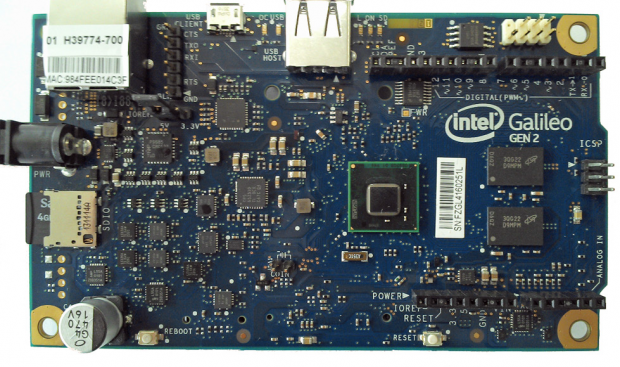
\includegraphics[height=5cm]{obrazky/embed_intel_galileo}
  \end{center}
	\vspace{-20pt}
  \caption{Intel Galileo~\cite{IntelGalileo}}
	\vspace{-10pt}
\end{figure}
		
		
		\subsection{Intel Edison} 
		Intel Edison je druhý jednočipový počítač architektury x86 vyvinutý společností Intel. Má velikost SD karty a je určený pro nositelnou elektroniku. Obsahuje dvoujádrový procesor Intel Quark x86 na frekvenci 400 MHz. Dále obsahuje 1\,GB RAM a 4\,GB flash paměti. Konektivita je zajištěna pomocí 70 pinového Hirose DF40 konektoru, který v sobě sdružuje veškerá dostupná rozhraní (USB, GPIO, SPI, I2C a~PWM). Jsou k dispozici dvě rozšiřující desky~\cite{IntelEdison}:
			
			\begin{itemize}
				\item Arduino board - Arduino board je plně kompatibilní s Arduinem, včetně podpory Arduino shieldů a modulů. Dále tato deska zpřístupňuje 20 digitálních I/O pinů, z toho 4 z nich lze využít jako PWM výstupy. Dále obsahuje 6 analogových vstupů, UART sběrnici, I2C sběrnici, SPI sběrnici. Dále obsahuje 2~USB konektory, jeden pro napájení, druhý připojený k UART sběrnici a slot na SD kartu.
				
				\begin{figure}[!ht]
  \begin{center}
    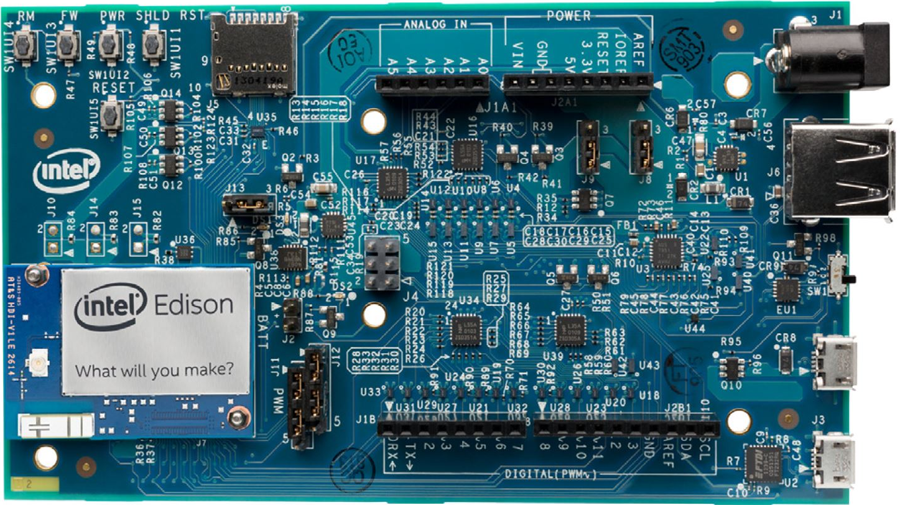
\includegraphics[height=4.5cm]{obrazky/embed_intel_edison2}
  \end{center}
	\vspace{-20pt}
  \caption{Arduino board pro Intel Edison}
	\label{embed_intel_edison2}
	\vspace{-10pt}
\end{figure}
				
				\item Intel breakout board -  Tato deska je díky svým malým rozměrům vhodná pro~prototypování nositelné elektroniky či pro Internet věcí. Obsahuje pájitelnou mřížku pro zpřístupnění věškerých dostupých rozhraní. Na desku jsou vyvedeny pouze dva USB konektory, jeden pro napájení a druhý připojený k UART sběrnici.
\end{itemize}

\begin{figure}[!ht]
  \begin{center}
    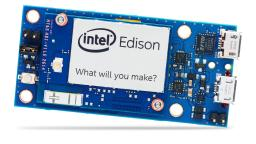
\includegraphics[height=2.5cm]{obrazky/embed_intel_edison1}
  \end{center}
	\vspace{-20pt}
  \caption{Intel breakout board}
	\label{embed_intel_edison1}
	\vspace{-10pt}
\end{figure}

Desky Intel se hodí spíše pro větší typy projektů, kdy již vývojové prostředí Arduina nestačí a je potřeba využít plného potenciálu operačního systému.

%%%%%%%%%%%%%%%%%%%%%%%%%%%%%%%%%%%%%%%%%%%%%%%%%%%%%%%%%%%%%%%%%%%%%%%%%%%%%%%%%%%%%%%%%%%%%%%%%%%%%%%%%%%%%%%%%
%%%%%%%%%%%%%%%%%%%%%%%%%%%%%%%%%%%%%%%%%%%%%%%%%%%%%%%%%%%%%%%%%%%%%%%%%%%%%%%%%%%%%%%%%%%%%%%%%%%%%%%%%%%%%%%%%
%%%%%%%%%%%%%%%%%%%%%%%%%%%%%%%%%%%%%%%%%%%%%%%%%%%%%%%%%%%%%%%%%%%%%%%%%%%%%%%%%%%%%%%%%%%%%%%%%%%%%%%%%%%%%%%%%
%%%%%%%%%%%%%%%%%%%%%%%%%%%%%%%%%%%%%%%%%%%%%%%%%%%%%%%%%%%%%%%%%%%%%%%%%%%%%%%%%%%%%%%%%%%%%%%%%%%%%%%%%%%%%%%%%
%%%%%%%%%%%%%%%%%%%%%%%%%%%%%%%%%%%%%%%%%%%%%%%%%%%%%%%%%%%%%%%%%%%%%%%%%%%%%%%%%%%%%%%%%%%%%%%%%%%%%%%%%%%%%%%%%
%%%%%%%%%%%%%%%%%%%%%%%%%%%%%%%%%%%%%%%%%%%%%%%%%%%%%%%%%%%%%%%%%%%%%%%%%%%%%%%%%%%%%%%%%%%%%%%%%%%%%%%%%%%%%%%%%

 \section{AMD Gizmo}
\label{KapAMD}

	Gizmo Board a Gizmo Board 2 od firmy AMD jsou alternativou k počítačům RaspberryPi, nabízející však platformu IBM PC a 64bitovou architekturu. Umožňuje tedy běh klasických operačních systémů, včetně Windows.
	
		\textbf{Gizmo Board 1} beží na dvoujádrovém APU G-T40E od firmy AMD na frekvenci 1GHz při příkonu 10\,W. Součástí procesoru je grafický čip Radeon HD 6250. K dispozici je 1\,GB RAM. Deska dále obsahuje dvojici USB, VGA, audio výstup, SATA a Ethernet konektor. Další sběrnice jako GPIO, SPI, I2C, UART a~PWM jsou dostupné po připojení rozšiřující karty přes LowSpeed~\cite{AmdGizmo1}.
	
	\textbf{ Gizmo Board 2} je vybaven APU AMD GX210HA na~frekvenci 1 GHz, s~integrovaným GPU AMD Radeon HD 8210E s frekvencí 300\,MHz. Příkon je 9\,W. Tento model má také 1\,GB RAM. Tato verze disponuje 4 USB, HDMI výstupem, MicroSD slotem a Ethernetovým portem. Mezi další rozhraní patří PCI Express (Peripheral Component Interconnect Express), GPIO, SPI, I2C, UART, DAC/ADC (Digital to Analog Converter/Analog to Digital Converter) nebo PWM \cite{AmdGizmo2}.


\begin{figure*}[!ht]
    \centering
			\subfigure[Gizmo Board 1]{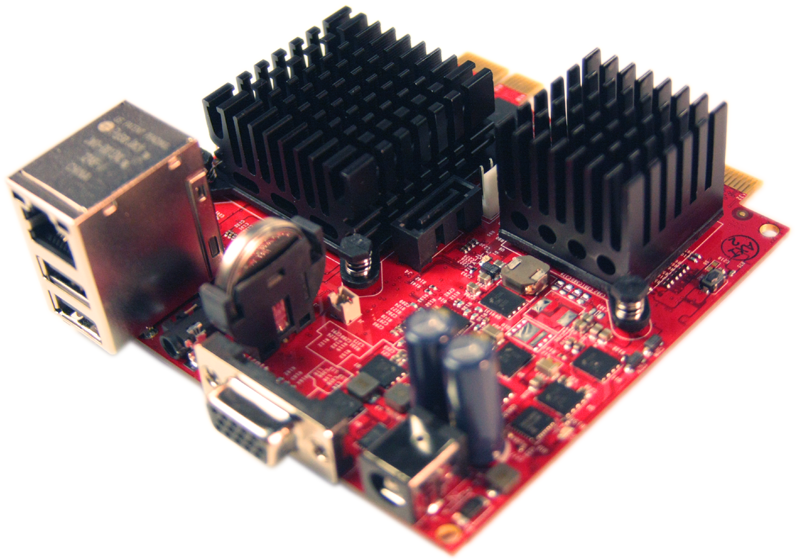
\includegraphics[width=0.45\textwidth]{obrazky/embed_amd_gizmo1}\label{embed_amd_gizmo1}}
			\hspace*{5mm}
			\subfigure[Gizmo Board 2]{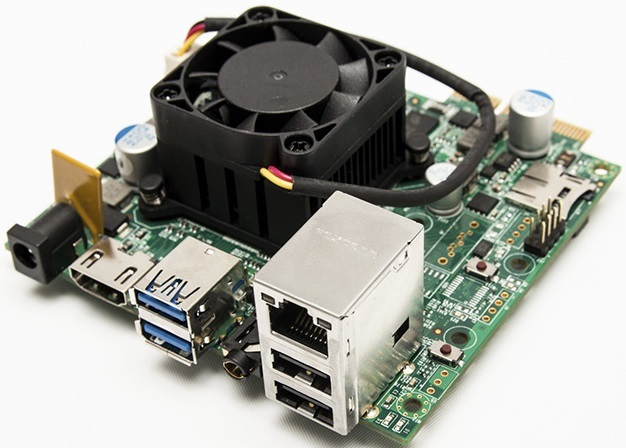
\includegraphics[width=0.45\textwidth]{obrazky/embed_amd_gizmo2}\label{embed_amd_gizmo2}}
		\caption{AMD Gizmo}
\end{figure*}



	
Oba počítače již poskytují dostatečný výkon pro embedded zařízení, avšak druhá verze zařízení již využívá aktivní chlazení a je hlučnější. Obě zařízení jsou větších rozměrů a nemají dostatečnou dokumentaci k přístupu a programování jednotlivých rozhraní. Hodí se spíše pro~aplikace jako multimediální centrum či jednodušší počítač, než pro IoT nebo~průmyslovou automatizaci. Komunita okolo AMD Gizmo prakticky neexistuje.
	
	



